\chapter{Background and Related Work}
\label{ch:background}

This chapter explains the concepts needed to understand our work. We start with what implicit neural representations are and how they work. Then we discuss the spectral bias problem that limits standard neural networks. Finally, we review the eight methods we evaluate in this thesis.

\section{Implicit Neural Representations}

\subsection{The Basic Idea}

An implicit neural representation uses a neural network to describe a shape as a continuous function. For three-dimensional occupancy, the network learns a function $f_\theta$ that takes any point in space $(x, y, z)$ and outputs a value between 0 and 1. This value tells us the probability that the point is inside the object. If the output is close to 1, the point is likely inside. If it is close to 0, the point is likely outside.

This approach differs from traditional methods in an important way. Instead of storing a grid of values that grows with resolution, we store the network's parameters. A network with a few hundred thousand parameters can represent shapes that would need billions of voxels. The network can also be queried at any resolution without retraining, since it defines a continuous function rather than discrete samples.

\subsection{Network Structure}

The function $f_\theta$ is typically implemented as a Multi-Layer Perceptron. Each layer takes an input, multiplies it by a weight matrix, adds a bias, and applies an activation function. Mathematically, layer $i$ computes:
\begin{equation}
    \mathbf{y}_i = \sigma(\mathbf{W}_i \mathbf{y}_{i-1} + \mathbf{b}_i)
\end{equation}
where $\sigma$ is the activation function, $\mathbf{W}_i$ is the weight matrix, and $\mathbf{b}_i$ is the bias vector. The network takes coordinates $(x, y, z)$ as input and produces an occupancy probability as output.

The activation function $\sigma$ plays a crucial role. Standard choices like ReLU create piecewise linear functions, which struggle to represent smooth curves and sharp details. This limitation motivates the architectural innovations we discuss later.

\subsection{Training the Network}

We train the network using Binary Cross-Entropy loss, which is well suited for classification tasks:
\begin{equation}
    \mathcal{L}_{\text{BCE}} = -\frac{1}{N} \sum_{i=1}^{N} \left[ o_i^* \log(o_i) + (1 - o_i^*) \log(1 - o_i) \right]
\end{equation}
Here, $N$ is the number of training points, $o_i^*$ is the true label (1 for inside, 0 for outside), and $o_i$ is the network's prediction. This loss penalizes confident wrong predictions heavily, encouraging the network to be accurate near object boundaries.

\section{The Spectral Bias Problem}

\subsection{What Goes Wrong}

Standard neural networks with ReLU activations have a fundamental limitation. When trained to represent shapes, they produce smooth, rounded outputs that miss sharp edges and fine details. This happens consistently across different shapes and training procedures.

Rahaman et al.~\cite{rahaman2019spectral} studied this problem and named it spectral bias. They found that neural networks learn low-frequency patterns quickly but struggle with high-frequency patterns. In practical terms, the network captures the overall shape early in training but makes little progress on fine details even after many iterations.

\subsection{Why It Happens}

The theoretical explanation involves how gradients flow during training. Jacot et al.~\cite{jacot2018ntk} showed that neural network training is governed by a mathematical object called the Neural Tangent Kernel. For ReLU networks, this kernel favors low frequencies. High-frequency components receive smaller gradient updates and therefore learn more slowly.

There is also an intuitive explanation. ReLU networks create piecewise linear functions. To represent a sharp edge, the network needs many small linear pieces arranged precisely. This requires careful coordination across many parameters, which gradient descent achieves slowly. The result is that sharp features remain blurry even after extensive training.

For three-dimensional occupancy, this bias causes several problems. Edges become rounded. Fine surface details disappear. Thin structures merge together. The boundary between inside and outside becomes blurred rather than sharp.

\section{Taxonomy of INR Methods}

Researchers have proposed many methods to overcome spectral bias. Following the classification by Essakine et al.~\cite{essakine2024inr}, we organize these methods into four categories based on their approach. Figure~\ref{fig:taxonomy} illustrates the architectural differences between categories.

\begin{figure}[htbp]
    \centering
    \begin{subfigure}[b]{0.45\textwidth}
        \centering
        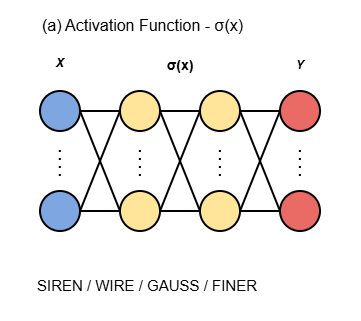
\includegraphics[width=\textwidth]{Figures/a.drawio.png}
        \caption{Category (a): Activation function enhancement. Methods like SIREN, WIRE, GAUSS, and FINER replace standard activations with functions designed for high-frequency content.}
        \label{fig:cat_a}
    \end{subfigure}
    \hfill
    \begin{subfigure}[b]{0.45\textwidth}
        \centering
        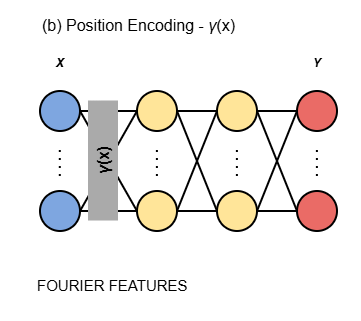
\includegraphics[width=\textwidth]{Figures/b.drawio.png}
        \caption{Category (b): Positional encoding. Fourier Features transforms coordinates before feeding them to a standard network.}
        \label{fig:cat_b}
    \end{subfigure}
    
    \vspace{0.5cm}
    
    \begin{subfigure}[b]{0.45\textwidth}
        \centering
        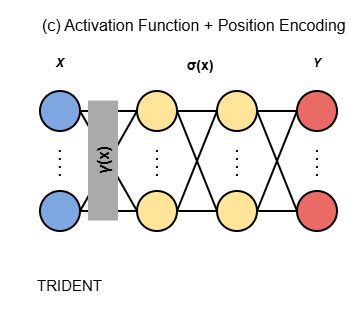
\includegraphics[width=\textwidth]{Figures/c.drawio.png}
        \caption{Category (c): Combined approach. TRIDENT uses both positional encoding and specialized activations.}
        \label{fig:cat_c}
    \end{subfigure}
    \hfill
    \begin{subfigure}[b]{0.45\textwidth}
        \centering
        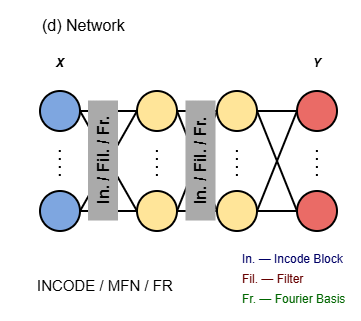
\includegraphics[width=\textwidth]{Figures/d.drawio.png}
        \caption{Category (d): Network structure optimization. INCODE, MFN, and FR modify how layers interact.}
        \label{fig:cat_d}
    \end{subfigure}
    \caption{Taxonomy of implicit neural representation methods. Each category takes a different approach to overcoming spectral bias. Blue nodes represent input coordinates, yellow nodes are hidden layers, and red nodes produce output values.}
    \label{fig:taxonomy}
\end{figure}

\newpage
\subsection{Category (a): Activation Function Enhancement}

The most direct approach replaces ReLU with activation functions better suited for high-frequency content. Four methods fall into this category.

\textbf{SIREN}~\cite{sitzmann2020siren} uses sine functions as activations: $\sigma(x) = \sin(\omega_0 x)$. The parameter $\omega_0$ controls the frequency. In our experiments, we use $\omega_0 = 30$ for both the first layer and the hidden layers. Sine functions are periodic and smooth, making them naturally suited for representing oscillating patterns. SIREN requires special weight initialization to work properly, but once configured correctly, it captures fine details much better than ReLU networks.

\textbf{GAUSS}~\cite{ramasinghe2022gauss} uses Gaussian activations: $\sigma(x) = \exp(-(sx)^2)$. The parameter $s$ controls the width. We use an input scale of 20.0 and $\sigma = 1.0$. Gaussians provide spatial localization, meaning each neuron responds to a limited region of input space. This property helps represent local features without affecting distant regions.

\textbf{WIRE}~\cite{saragadam2023wire} uses Gabor wavelets, which combine Gaussian localization with sinusoidal oscillation: $\sigma(x) = \exp(-(sx)^2 + i\omega x)$. This complex-valued activation achieves optimal localization in both space and frequency according to the uncertainty principle. We use $\omega_0 = 40$ for the first layer, $\omega_0 = 20$ for hidden layers, and $\sigma_0 = 3.0$. WIRE requires special handling for complex numbers during training.

\textbf{FINER}~\cite{liu2024finer} extends SIREN by making the frequency depend on input: $\sigma(x) = \sin(\omega_0(|x| + 1) \cdot x)$. This allows different neurons to operate at different frequencies based on what they need to represent. We use 16 frequency bands. Regions with fine detail can use high frequencies while smooth regions use low frequencies.

\subsection{Category (b): Positional Encoding}

Instead of changing activations, positional encoding transforms the input coordinates before processing. The idea is to map low-dimensional inputs into a higher-dimensional space where high-frequency patterns become easier to learn.

\textbf{Fourier Features}~\cite{tancik2020fourier} projects coordinates through random sinusoids:
\begin{equation}
    \gamma(\mathbf{x}) = [\cos(2\pi\mathbf{B}\mathbf{x}), \sin(2\pi\mathbf{B}\mathbf{x})]^\top
\end{equation}
where $\mathbf{B} \in \mathbb{R}^{3 \times m}$ is a random matrix sampled from $\mathcal{N}(0, \sigma^2)$ and fixed at initialization. Two easily confused parameters govern the encoding: $m$, the \emph{number} of random frequencies, which sets the encoded width $2m$; and $\sigma$, the \emph{scale}, which determines how high those frequencies reach. We use $m = 256$ and $\sigma = 1.0$. Chapter~\ref{ch:results} shows that $\sigma$ is the single most consequential hyperparameter in this study. After this transformation, even a standard ReLU network can learn high-frequency functions.

\subsection{Category (c): Combined Approaches}

Some methods combine positional encoding with specialized activation functions, aiming to get the benefits of both approaches.

\textbf{TRIDENT} uses both a positional encoding layer $\gamma(x)$ and specialized activation functions $\sigma(x)$ throughout the network. As shown in Figure~\ref{fig:cat_c}, coordinates first pass through a positional encoding transformation, then through layers with non-standard activations. This combination can potentially capture a wider range of frequencies than either approach alone. However, it also introduces more hyperparameters to tune and increases computational cost. We do not evaluate TRIDENT in this thesis but include it in our taxonomy for completeness.
\subsection{Category (d): Network Structure Optimization}

These methods change how layers are organized or how they interact, rather than modifying individual components.

\textbf{INCODE}~\cite{kazerouni2024incode} uses a helper network called a harmonizer to adjust activation parameters during training. The main network uses modulated sine activations: $\sigma(x) = a \sin(b\omega_0 x + c) + d$. The parameters $a, b, c, d$ are predicted by the harmonizer based on the input. We use a scale of 50.0. This allows the network to adapt its behavior to different regions of the shape.

\textbf{MFN}~\cite{fathony2021mfn} (Multiplicative Filter Networks) replaces addition with multiplication between layers: $\mathbf{y}_i = \sigma(\mathbf{W}_i \mathbf{y}_{i-1}) \odot \sigma(\mathbf{V}_i \mathbf{x})$. The symbol $\odot$ denotes element-wise multiplication. We use input scale 10.0, $\alpha = 6.0$, and $\beta = 1.0$. This creates complex frequency interactions but, as we will show, can cause problems at sharp boundaries.

\textbf{FR}~\cite{shi2024fr} (Fourier Reparameterized) encodes frequency information in the weight matrices themselves. The weights are parameterized through learnable coefficients applied to Fourier basis functions. We use $F = 64$ frequencies. This encourages the network to develop frequency-aware representations.

\section{Key Architectural Properties}

Essakine et al.~\cite{essakine2024inr} identified three properties that help predict how well a method will perform. Understanding these properties guides method selection.

\textbf{Spatial compactness} means the network can represent local features without affecting distant regions. When a spatially compact network learns a feature in one area, it does not disturb what it has learned elsewhere. Most methods except Fourier Features, MFN, and FR have this property.

\textbf{Frequency compactness} means the network can isolate specific frequency ranges without leakage into other frequencies. This is important for representing sharp boundaries, which require precise high-frequency content. GAUSS, WIRE, FINER, and INCODE have this property.

\textbf{Adaptivity} means the network can adjust its behavior based on what it needs to represent. Adaptive methods can allocate more capacity to complex regions and less to simple ones. FINER, INCODE, and FR have this property.

Table~\ref{tab:properties} summarizes which methods have which properties. Our experiments examine whether these properties predict reconstruction quality for three-dimensional occupancy, and how robust any such relationship is.

\begin{table}[htbp]
\centering
\caption{Properties of each method according to the taxonomy of Essakine et al.~\cite{essakine2024inr}.}
\label{tab:properties}
\begin{tabular}{lcccc}
\toprule
\textbf{Method} & \textbf{Category} & \textbf{Spatial} & \textbf{Frequency} & \textbf{Adaptivity} \\
\midrule
SIREN & (a) & \checkmark & $\times$ & $\times$ \\
GAUSS & (a) & \checkmark & \checkmark & $\times$ \\
WIRE & (a) & \checkmark & \checkmark & $\times$ \\
FINER & (a) & \checkmark & \checkmark & \checkmark \\
Fourier Features & (b) & $\times$ & $\times$ & $\times$ \\
INCODE & (d) & \checkmark & \checkmark & \checkmark \\
MFN & (d) & $\times$ & $\times$ & $\times$ \\
FR & (d) & $\times$ & $\times$ & \checkmark \\
\bottomrule
\end{tabular}
\end{table}

\section{Occupancy Networks}

The idea of using neural networks to represent shapes as occupancy functions comes from Mescheder et al.~\cite{mescheder2019occupancy}. Their Occupancy Networks paper showed that implicit functions provide a natural way to represent three-dimensional shapes without the limitations of voxels or meshes.

Given a shape $S$, the occupancy function returns 1 for points inside the shape and 0 for points outside. During training, we sample points throughout space and teach the network to classify them correctly. At test time, we can query the network at any resolution. To extract a mesh, we evaluate the network on a dense grid and use the Marching Cubes algorithm~\cite{lorensen1987marching} to find the surface where occupancy equals 0.5.

This representation handles complex topology naturally. Shapes with holes, multiple parts, or intricate detail all work the same way. However, the sharp transition between inside and outside places strong demands on the network's ability to represent high-frequency content. This makes the choice of architecture particularly important for occupancy prediction.

